\documentclass{article}

\usepackage[scaled]{helvet}
\renewcommand\familydefault{\sfdefault} 
\usepackage[T1]{fontenc}
\usepackage{fancyhdr}
\usepackage{graphicx}
\usepackage{subfigure}
\usepackage{booktabs}
\usepackage[inline]{enumitem}
\usepackage{float}

\usepackage{amsmath}

\usepackage{hyperref}
\hypersetup{
    colorlinks=true,
    citecolor=[RGB]{0,0.5,0.5},
    urlcolor=[RGB]{0,0.5,0.5},
    linkcolor=[RGB]{0,0.5,0.5}
}

\usepackage{geometry}
\geometry{margin={0.8in,1in}}

\usepackage[colorinlistoftodos,prependcaption,textsize=small]{todonotes}

\begin{document}

\begin{centering}
\Large\textbf{{\sc CMPT 423-820 Mini Project 3 Report}}\\[1ex]
\begin{center}
\small{Alireza Falamarzi (ylw576), Baptiste Rouquette (dly490), Princess Tayab (prt898), Talha Mansoor (kgy284)}
\end{center}
\end{centering}
\hrule

\vspace{0.1in}
\section{Line Plot: Decrease in Distortion as the K Hyperparameter Increases}
\begin{figure}[H]
    \centering
    \vspace{-10pt}
    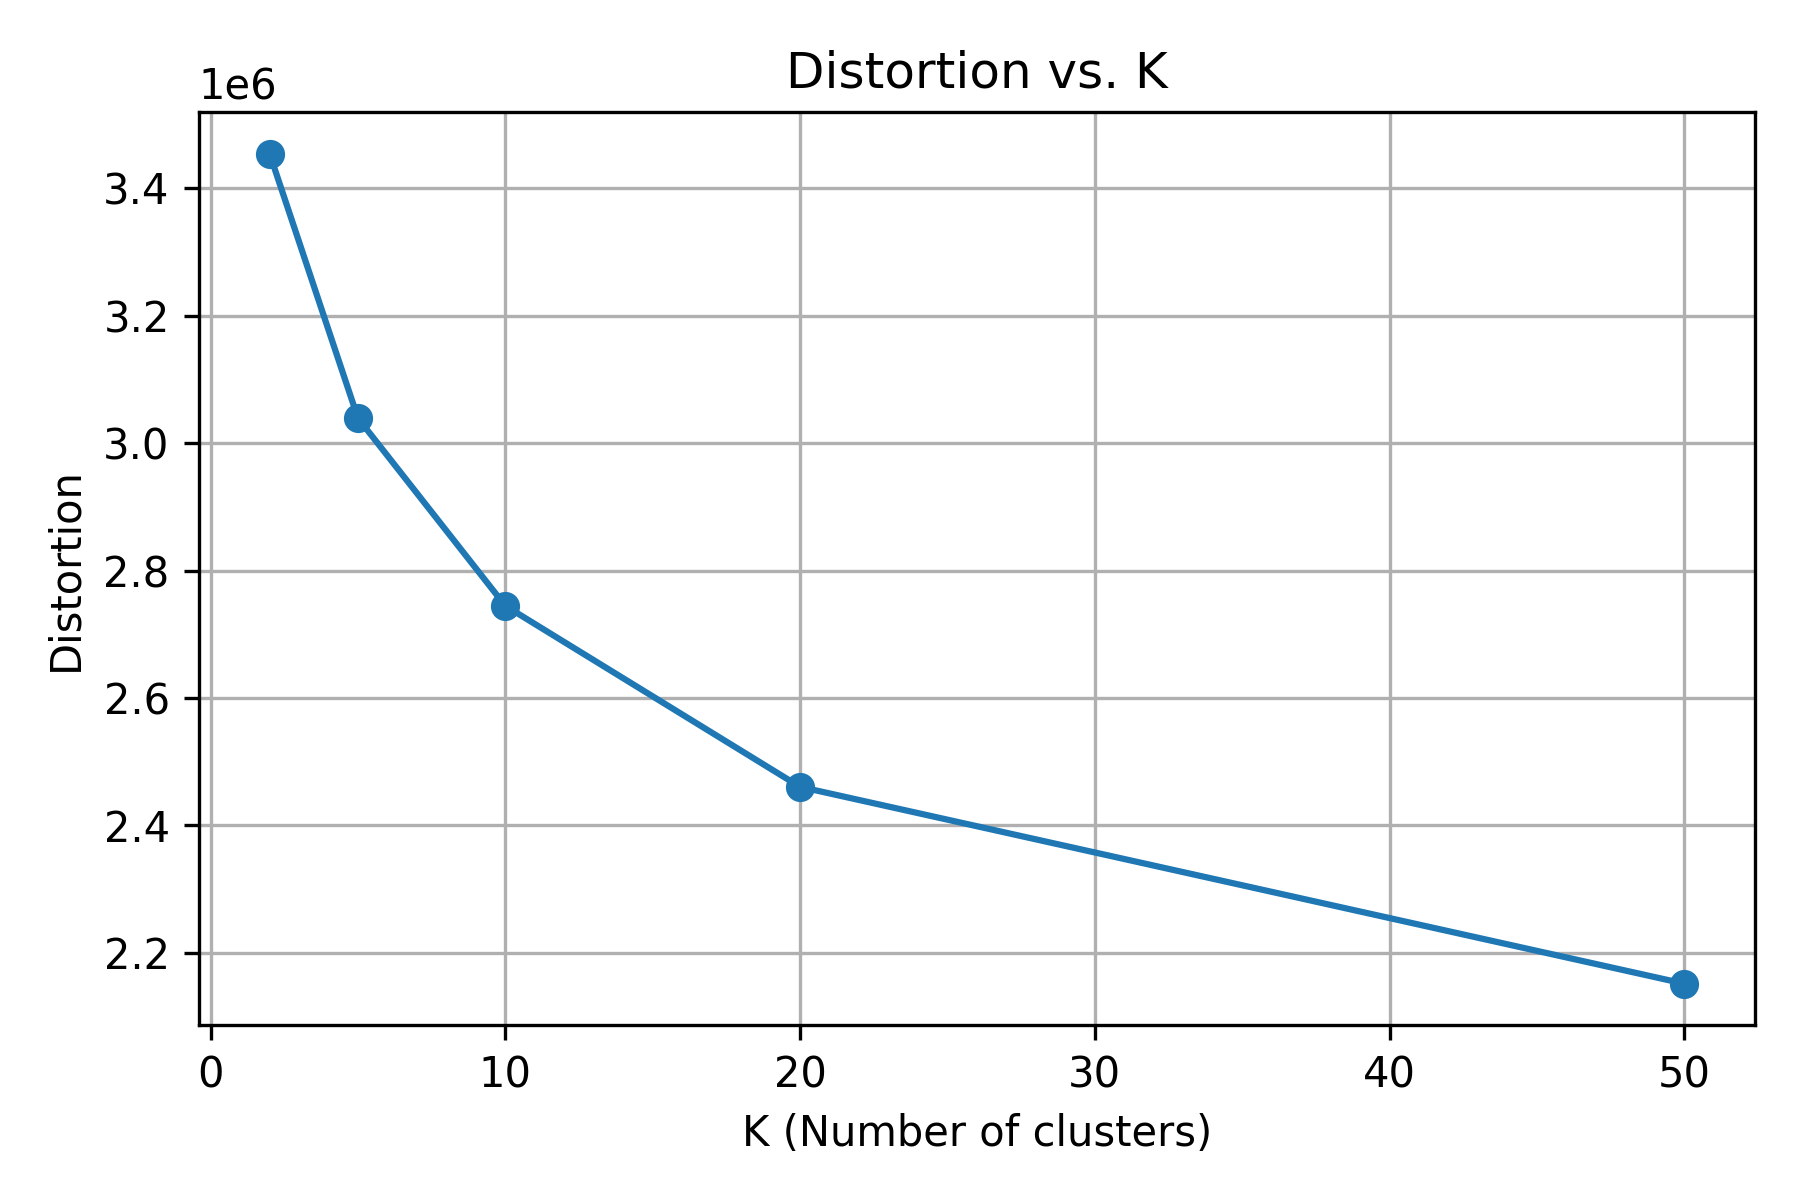
\includegraphics[width=0.6\textwidth]{figure/distortion_vs_k.png} 
\end{figure}
\vspace{-15pt}
\begin{center}
    Distortion decreases as \( K \) increases, with diminishing returns.
\end{center}


\section{Cluster Centroid Visualization}

\begin{figure}[H]
    \centering
    
\includegraphics[width=1\textwidth]{figure/outputk50a.png} 
    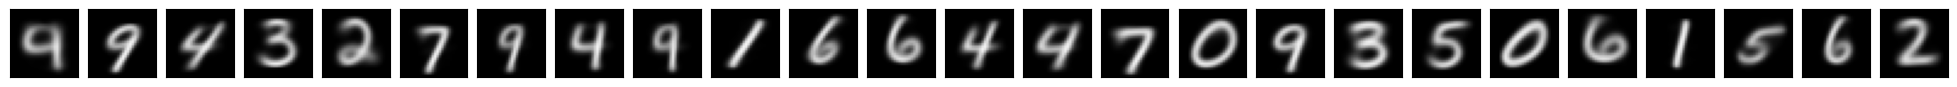
\includegraphics[width=1\textwidth]{figure/outputk50b.png} 
    \vspace{-25pt} 
    \caption{k = 50}
\end{figure}
\vspace{-10pt} 
\begin{figure}[H]
    \centering
    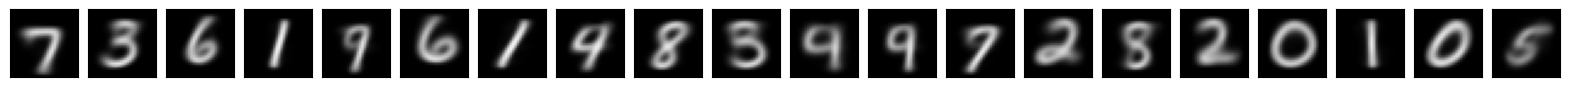
\includegraphics[width=1\textwidth]{figure/outputk20.png} 
    \vspace{-25pt} 
    \caption{k = 20}
\end{figure}
\vspace{-10pt} 
\begin{figure}[H]
    \centering
    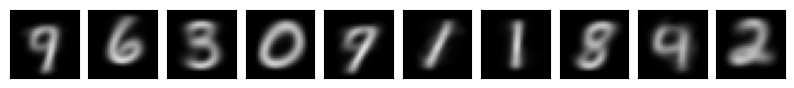
\includegraphics[height=1.5cm]{figure/outputk10.png} 
    \vspace{-15pt} 
    \caption{k = 10}
\end{figure}
\vspace{-10pt} 
\begin{figure}[H]
    \centering
    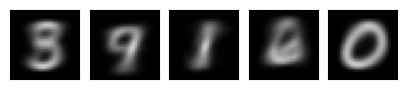
\includegraphics[height=1.5cm]{figure/outputk5.png} 
    \vspace{-15pt} 
    \caption{k = 5}
\end{figure}
\vspace{-10pt} 
\begin{figure}[H]
    \centering
    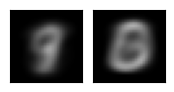
\includegraphics[height=1.5cm]{figure/outputk2.png} 
    \vspace{-15pt} 
    \caption{k = 2}
\end{figure}

\paragraph{How does the k parameter influence finding all
10 digit classes?}
\begin{itemize}
    \item Figure 1: All 10 digits appear multiple times.
    \item Figure 2: All digits appear at least once.
    \item Figure 3: Some digits are clearly missing such as 5 and 7 with some ambiguity between 3/8 and 4/9
    \item Figure 4: Majority of the digits are missing. 0,1, and 9 digits are the only digits that appear clearly and possibly 3.
    \item Figure 5: No digits appear clearly. Each cluster could be described as multiple numbers.
\end{itemize}

\paragraph{Does each cluster contain images of one or multiple digits?}
\begin{itemize}
    \item Figure 1: Most clusters contain only one image. Possibly leading to oversegmentation with some ambiguity between digits like 9 and 4. One cluster is extremely confused (multiple clusters for the same digit).
    \item Figure 2: Clusters become less defined than with k=50 and most clusters show one image digit. There are some still mixed multiple digits, particularly showing confusion between 4/9 (again) and 3/8.
    \item Figure 3: Most digits have a single main cluster, but the separation isn't as sharp as with k=20, and the 4/9 confusion persists.
    \item Figure 4: Clusters now group multiple digits together, but some structure emerges. For example, "1" (a simple straight line) is easier to distinguish, but most other digits are mixed.
    \item Figure 5: Severe mixing occurs where each cluster has multiple images resulting with no meaningful digit-specific clusters.
\end{itemize}

\section {The Effectiveness of K-Means Clustering in Identifying 10 Digit Classes in the MNIST Dataset}
K-Means clustering tries to group the digits in the MNIST dataset but has trouble separating them clearly because it only looks at pixel similarities, and digits can look very similar even if they belong to different classes. For example, digits like 1 and 7 or 3 and 5 have similar shapes or overlapping features, which confuses the algorithm. K-Means doesn’t consider the actual digit labels and groups based on overall pixel structure, so it sometimes mixes up visually similar digits, like 4 and 9, or 3, 5 and 8, even though they are distinct. The number of clusters, or "k," really affects how well it works. With a high k (like k=50), the algorithm ends up splitting the same digit into multiple clusters, but it still struggles with digits that look similar. At k=10, which matches the number of digit classes, it’s still not perfect as some digits are missing or mixed up because of overlapping features. Lower k values (like k=5 or k=2) end up grouping too many digits together, losing important differences. The main issue is that K-Means relies on measuring straight-line distance between pixels and doesn’t take labels into account, so even if the distortion is reduced with a higher k, it doesn’t necessarily improve digit separation. By testing clustering with different k values, we can see how unsupervised learning can reveal some structure in the digit images. However, K-Means isn’t guaranteed to produce meaningful clusters without supervision, as shown by missing or combined digit representations. 





\end{document}